
% this file is called up by thesis.tex
% content in this file will be fed into the main document

%: ----------------------- introduction file header -----------------------
\chapter{Scalable Creation and Inference of Topics}\label{ch:scalability}

\graphicspath{{scalability/figures/}}

% -------------------------------------------------------------
% -- Scalability
% -------------------------------------------------------------

Given the huge amount of textual data daily produced in multiple domains and the limited availability of resources, it becomes crucial to provide efficient mechanisms for managing this raw data to make sense of it. This chapter presents a framework for processing probabilistic topics in collections ranging from only a few hundred documents, to thousands or even millions of texts. The methods and algorithms proposed in this thesis have been implemented and evaluated in this environment, which therefore serves as the technological basis for our research. The motivation is twofold, on the one hand to create a scalable system to analyze documents and discover topics, and on the other hand to create reusable topic models that can easily be integrated into that environment.


\section{Distributed Platform for Document Analysis}

% existentes herramientas de análisis de textos: escalabilidad vertical

While some of the algorithms that support NLP tasks allow for advanced sense-making operations (e.g sentiment analysis, document clustering), others are focused on fundamental tasks such as NER, PoS tagging or stemming, that are usually combined into more complex operations (e.g topic modeling). However, integrating these algorithms involves significant efforts on reconciling their implementations, coordinating processing operations and efficiently exploiting results coming from multiple formats. A more standardized approach that is open to different implementation technologies and data formats, maximizes their reuse and facilitates the scalability of the processing pipeline. Reuse is increased by reducing integration problems resulting from proprietary data formats and incompatible technology stacks. The use of the algorithms and their results are unified. The (horizontal) scalability is also benefited by being able to build distributed solutions that combine their results in a homogeneous way. 

We propose a distributed workflow where multiple and heterogeneous NLP tools can work together from isolated and high-performance environments to compose a global pipeline shared by all. The tasks instead of following a sequence of steps emerge as a result of the combination of actions. This raises both technical and functional challenges to coordinate multiple executions. From the technical point of view, isolated environments and communication mechanisms are provided so dissimilar tools can be executed with maximum guarantees. From the functional point of view, all executions are coordinated to reach a final result as aggregation of partial results derived from each execution.


\subsection{Text-oriented Model}

There are three key elements whose interactions guide the execution of the workflow: \textit{resources}, \textit{actions} and \textit{states}. A resource can be a \textit{document} (e.g. a research paper), a \textit{part-of} another resource (e.g. a section of a document), a \textit{domain} (e.g. a journal) or an \textit{annotation} (e.g. a topic). An action is any operation performed on a resource (e.g. \textit{create}, \textit{update} or \textit{delete}). A state is reached by a resource after an action is performed (e.g. \textit{created}, \textit{updated} or \textit{deleted}). Let's see an example to better understand the approach. , consider the research papers published at the SIGGRAPH conference in 2016\footnote{http://s2016.siggraph.org}. First, every paper is materialized as a new \textit{document} containing its full-text. Then, every \textit{document} is automatically related to several \textit{parts}, each of them grouping sentences by rhetorical class (e.g. approach, background, challenge, future work and outcome) and by section (e.g abstract, introduction, conclusion). Finally, a new \textit{domain} is created grouping all these \textit{documents}. Different analysis can be performed extending the initial set of resources with more annotations at several representational levels: at \textit{document level}, full-text based annotations are provided such as named-entities, compounds and descriptive tags. At \textit{relational level}, connection between resources are found (e.g. semantic similarity-based relationships). And finally, at \textit{domain level} annotations such as tags and summaries are composed describing the corpus of \textit{documents}.

\textit{Resources}, \textit{actions}, \textit{states} are individually addressable and linkable \cite{Turchi2012a} following the Linked Data principles defined by T. Berners-Lee \cite{Bizer2009}. Thus, resources (i.e. a \textit{domain}, a \textit{document}, a \textit{part-of} or an \textit{annotation}) have:
(1) a URI as name, (2) a retrievable (or dereferenceable) HTTP URI so that it can be looked up, (3) a useful information provided by using standard notation (e.g. JavaScript Object Notation (JSON)) when it is  looked up by URI, and (4) links to other URIs so that other resources can be discovered from it.


There is an additional element, \textbf{event}, which allows the notification of new actions performed on resources. They are broadcast so that any module subscribed to the workflow is aware of the changes made to the resources. This will, in turn, allow that any module can perform actions on one or more resources in response to a new state reached by a given resource. Actions that will be executed in parallel through distributed environments.

\begin{figure}
  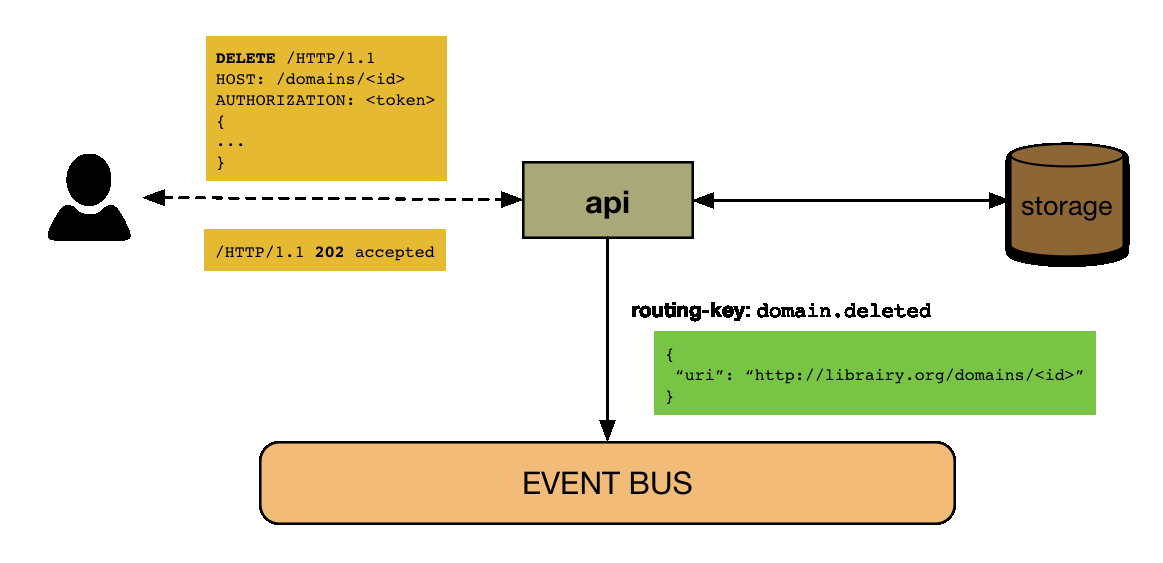
\includegraphics[scale=0.35]{api-domain-deleted}
  \caption{Domain deleted flow.}
  \label{fig:librairy-domain-deleted}
\end{figure}

An event illustrates a performed action, i.e. a resource and its new state, and follows the Representational State Transfer (REST)\cite{Fielding2002} paradigm. It takes into account the state reached after an action, i.e \textit{created}, \textit{deleted} or \textit{updated}. Thus, an event contains the resource type and the new state reached by a specific resource.


\subsection{Event-driven Workflow}
Following a publisher/subscriber approach, modules in the framework can publish and read \textit{events} to notify and to be notified about the state of a \textit{resource}. For example, when a new \textit{domain} is created, an \textit{event} message is published to the channel: $domain.created$. This \textit{event} could be managed by one or more modules which will be ready to perform and action (e.g. create a topic model) by using the \textit{documents} related to that \textit{domain}. 
Therefore, the system flow is not unique and is not explicitly implemented, instead distributed and emergent flows can appear according to particular actions on resources.

We use the Advanced Message Queuing Protocol (AMQP) as the messaging standard to avoid any cross-platform problem and any dependency to the selected message broker. This protocol defines: \textit{exchanges}, \textit{queues}, \textit{routing-keys} and \textit{binding-keys} to communicate publishers and consumers. A message sent by a publisher to an exchange is tagged with a routing-key. Consumers matching that routing-key with the binding-key used to link the queue to that exchange will receive the message. This key follows the structure: \textit{resource.status}. Since a wildcard-based definition can be used to set the key, this paradigm allow modules both listening to individual type events (e.g. \'domains.created\' for new domains), or multiple type events (e.g. \#.created for all new resources).

An \textit{event} can not only contain a string of characters in JSON format (default mode), but also an array of bytes serialized in a specific way. The type of the \textit{event}, i.e. its routing-key, implicitly defines the format (and serialization) of the message to be understood by both producers and consumers. 


\begin{figure}
  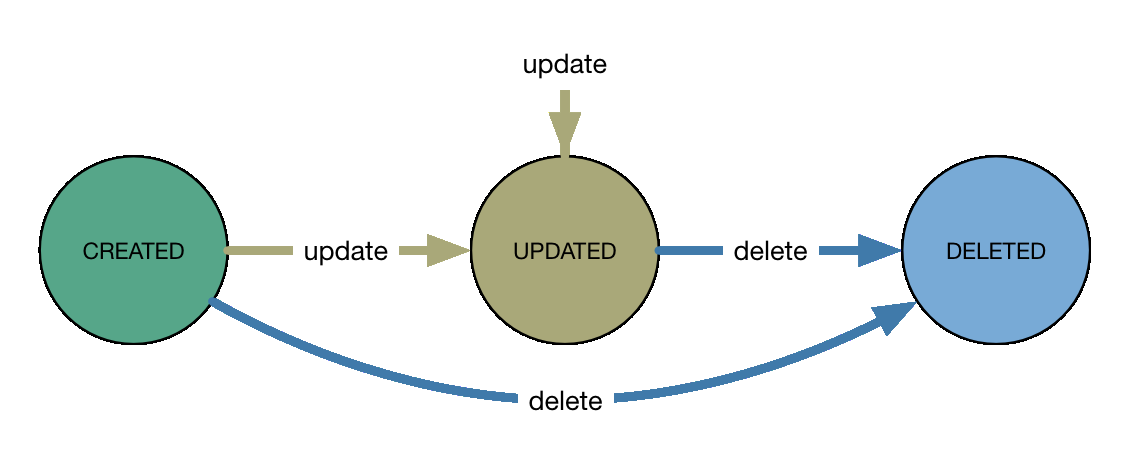
\includegraphics[scale=0.3]{resource-states}
  \caption{Resource states.}
  \label{fig:librairy-states}
\end{figure}

A HTTP-Rest Application Program Interface (API) was designed for interaction with end-users. Any external operation motivated by a user will be handled here. Some of them, usually those related to reading operations, will be completely managed by this module getting all the data from the internal storage. However, those operations implying a modification of the status of some resource (e.g. creation of a \textit{document}), may be also performed by other modules listening for that type of event asynchronously. This module publishes to the following routing-keys: \textit{domain.(created;updated;deleted)}, \textit{document.(created;updated;deleted)}, \textit{part.(created;updated;deleted)}, and \textit{annotation.(created;updated;deleted)}.

\subsection{Microservice Architecture}
A module is a processing unit that reacts to events generated from resources. They have been designed following the microservices architectural style. A module is a cohesive (i.e. it implements only functionalities strongly related to the concern that it is meant to model \cite{Dragoni2016}) and independent process working on the framework with a specific purpose. This purpose is defined by both the routing-key and the binding-key associated to the events handled by the module. 

These are three main types of modules:
\begin{itemize}
	\item \textbf{Harvester}: creates resources such as \textit{documents}, \textit{parts-of} and \textit{domains}, from local or remote located textual files.
    \begin{itemize}[rightmargin=\dimexpr\linewidth-5cm-\leftmargin\relax]
    	\item Listening for: nothing
		\item Publishing to: \textit{document.(created)}, 
        \textit{part.(created)}, \textit{domain.(created;updated)}
    \end{itemize}
    \item \textbf{Annotator}: retrieves named-entities, compounds, lemmas and other annotations resulting of Natural Language Processing (NLP) task execution from \textit{documents} and \textit{parts}.
    \begin{itemize}[rightmargin=\dimexpr\linewidth-5cm-\leftmargin\relax]
    	\item Listening for: \textit{document.(created;updated)}, \textit{part.(created;updated)}
		\item Publishing to: \textit{annotation.(created;deleted)}
    \end{itemize}
    \item \textbf{Modeler}: builds representational models from a given \textit{domain}. 
    \begin{itemize}[rightmargin=\dimexpr\linewidth-5cm-\leftmargin\relax]
    	\item Listening for: \textit{domain.(created;updated)}
		\item Publishing to: \textit{annotation.(created;deleted)}
    \end{itemize}
\end{itemize}

\begin{figure}
  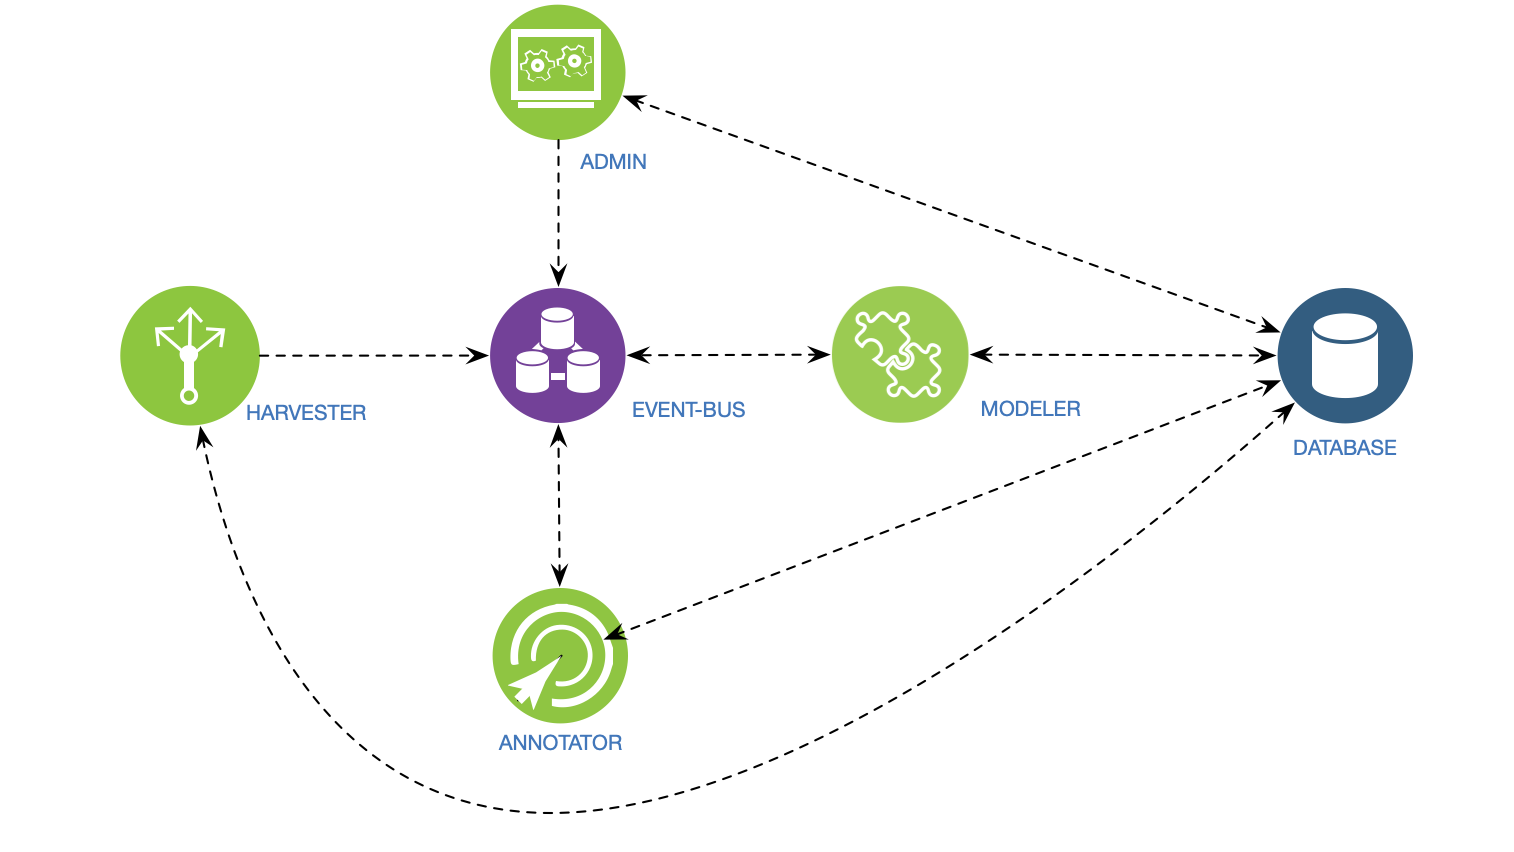
\includegraphics[scale=0.25]{modules}
  \caption{Modules.}
  \label{fig:librairy-modules}
\end{figure}



\section{Topic Model Service}
%present restful services to exploit a topic model
% topic-model-as-a-service

 


%\subsubsection{Storage}

%Multiple types of data can be handled in this ecosystem. Inspired in the Data Access Object (DAO) pattern, we have created a Unified Data Manager (UDM) providing access to any type of data used in the system.  Three types of databases have been considered:
%\begin{itemize}
	%\item \textbf{column-oriented database}: Focused on unique identified and/or \textit{structured data}. This storage allow %us searching key elements across resources. 
	%\item \textbf{document-oriented database}: Focused on indexing raw text. This storage allow us to execute advanced search %operations over all the information gathered about a textual resource. 
    %\item \textbf{graph database}: Focused on relations. This storage allow us exploring resources through the relationships %between them.
%\end{itemize}


\section{Summary}

A distributed framework is proposed where existing algorithms and tools coming from different technologies can work collaboratively to process and analyze huge collections of textual resources. This approach has been successfully applied to some real world scenarios \footnote{\url{http://drinventor.dia.fi.upm.es}}.
 
A new model definition based on the previously mentioned principle of maximizing information re-usability and minimize irrelevant data has been studied to create a fine-grained resource design. New domains, in the sense of particular vocabularies or specific textual formats, have been also analyzed to be included into the system via specific harvesters or more precise annotators. Moreover, a template-based mechanism oriented to facilitate the integration of new tools and techniques into the system has been built to make easier to develop new modules as well as increasing the available modules in public repositories.